\chapter{Theoretical framework}
\section{The Standard Model of particle physics}
The Standard Model of particle physics is a renormalisable quantum field theory based on gauge invariance principles.
At its core, the Standard Model postulates a set of elementary particles, divided into fermions, with half-integer spin and bosons, with integer spin,
and describes their interactions through three of the four fundamental forces: electromagnetism, the weak nuclear force, and the strong nuclear force.

The fundamental interactions obey a local gauge symmetry, which is associated to a Lie group $U(1)_Y \otimes SU(2)_T \otimes SU(3)_C$, where Y, T and C denote hypercharge, weak isospin and colour.

The interactions are mediated by gauge bosons such as the photon, the W and Z bosons and the gluons.
The strong interaction is governed by quantum chromodynamics (QCD), a gauge field theory based on colour symmetry group $SU(3)_C$,
and its eight generators correspond to the gluons.
The electroweak interaction is described by a gauge filed theory that is invariant under both weak isospin $I_3$ and hypercharge $Y$,
corresponding to the group $U(1)_Y$ $\otimes SU(2)_T$;
the electroweak interaction encompasses both electromagnetic and weak nuclear interactions,
mediated by the photon and by the W$^+$, W$^-$ and Z$^0$ boson respectively,
which come from the mixing of the generators of the two groups, as explained later in Section \ref{EWSB}.
The fundamental bosons all have spin 1, except for the Higgs Boson, which is the only known fundamental particle with spin 0.

Matter is described in the SM by twelve fermion fields.
All of the fundamental fermions have spin $\frac{1}{2}$ and include quarks, which constitute protons and neutrons, as well as leptons like electrons and neutrinos.
Quarks and leptons are further divided into three generations, each with two particles with different weak isospin, for a total of twelve elementary particles, as detailed in Table \ref{tab:fermions}; each fermion has a corresponding antiparticle with the same mass and spin and opposite charges for the three gauge groups.
Fermions belonging to different generations have different masses, which are not predicted by the model and must be determined experimentally.

The colour charge is exclusive to quarks, that carry a colour, and anti-quarks, which carry an anti-colour, while leptons and bound states with no net colour charge are called ``white''.
Similarly, gluons carry both a colour and an anti-colour charge, while all the other bosons are white.
Colour charge can exist in three states, arbitrarily labelled blue, green, and red, complemented by an anti-colour, anti-blue, anti-green, and untried.

Only the W$^+$ and the W$^-$ bosons carry electromagnetic charge, while the others are neutral.
Only left-handed fermions and right handed anti-fermions can be engaged in charged weak interactions, while the neutral weak interaction can involve both types, although with different couplings.

The Standard Model has not only successfully described a wide range of experimental observations but has also guided the discovery of new particles, like the Higgs boson, which was observed at the Large Hadron Collider in 2012 \cite{ATLASHiggsDiscovery, CMSHiggsDiscovery}.
This framework plays a pivotal role in our comprehension of the universe, spanning from the conditions just moments after the Big Bang to the inner workings of atomic nuclei.

\begin{table}[tbh]
	\centering
	\caption{Fundamental fermions, classified by family.}
	\label{tab:fermions}
	\begin{tabular}{ c c c c }
		\toprule
		 & 1$^{\text{st}}$ gen. & 2$^{\text{nd}}$ gen. & 3$^{\text{rd}}$ gen. \\%& Electric charge\\
		\midrule
		\multirow{2}{*}{Quarks}  & u       & c         & t          \\%& +$\dfrac{2}{3}$ \\
		                         & d       & s         & b          \\%& -$\dfrac{1}{3}$ \\
		\hline
		\multirow{2}{*}{Leptons} & $\nu_e$ & $\nu_\mu$ & $\nu_\tau$ \\%& 0              \\
		                         & e$^-$   & $\mu$$^-$ & $\tau$$^-$ \\%& -1             \\
		\bottomrule
	\end{tabular}
\end{table}

\begin{table}[th]
  \centering
  \caption{Hypercharge (Y), weak isospin (T$_3$) and electric charge (Q) of fermions. In the table below U and D mean any of the up-type (u,c,t) and down-type (d,s,b) quark, respectively.}
  \label{tab:charges}
  \begin{tabular}{ c c c c }
    \toprule
    & T$_3$ & Y & Q \\
    \midrule \addlinespace
    ${\dbinom{U}{D}}_L$             & $\dbinom{\frac{1}{2}}{-\frac{1}{2}}$ & $\dbinom{\frac{1}{3}}{\frac{1}{3}}$ & $\dbinom{\frac{2}{3}}{-\frac{1}{3}}$ \\ \addlinespace
    $u_R\, ,\  d_R$                 & $+\dfrac{4}{3}\, ,\  -\dfrac{2}{3}$  & $0\, ,\ 0$                          & $+\dfrac{2}{3}\, ,\  -\dfrac{1}{3}$  \\ \addlinespace
    \hline \addlinespace
    ${\dbinom{\nu_\ell}{\ell^-}}_L$ & $\dbinom{\frac{1}{2}}{-\frac{1}{2}}$ & $\dbinom{-1}{-1}$                   & $\dbinom{0}{-1}$                     \\ \addlinespace
    $u_R\, ,\  d_R$                 & $+\dfrac{4}{3}\, ,\  -\dfrac{2}{3}$  & $0\, ,\ 0$                          & $+\dfrac{2}{3}\, ,\  -\dfrac{1}{3}$  \\ \addlinespace
    \bottomrule
  \end{tabular}
\end{table}

\section{Electroweak Symmetry Breaking}
\label{EWSB}
Electromagnetic and weak interactions can be described as a unified electroweak interaction at high energies, mediated by massless bosons B, that generates U(1)$_Y$, and W$^{1, 2, 3}$, generators of SU(2)$_T$.
However, while experiments show that weak interactions are mediated by massive bosons, the inclusion of a mass term of the form $-\frac{1}{2} M^2 W^a_\mu W^{a\, \mu}$ violates the U(1) $\otimes$ SU(2) gauge invariance.
Moreover, the addition in the Lagrangian of a mass term to fermions in the form $-m_q \bar\psi \psi$ would violate the SU(2) invariance, since the left and right handed components of the field $\psi$ behave differently under such gauge transformation.

In the SM, the Electroweak Symmetry Breaking (EWSB), through the Brout-Englert-Higgs Mechanism, shortly called Higgs Mechanism, generates mass terms for gauge bosons while preserving gauge invariance.
The core idea is the spontaneous symmetry breaking, a concept originally elaborated in condensed matter physics.
In 1964 Brout and Englert \cite{PhysRevLett.13.321} and Higgs \cite{PhysRevLett.13.508, HIGGS1964132}

The EWSB causes also a mixing of the gauge boson fields, resulting in:
\begin{equation}
\begin{split}
  \PWpm &= \dfrac{1}{\sqrt{2}} \left( \PW^1 \mp \PW^2 \right)
  \\
  \begin{pmatrix} \PGg \\ \PZz \end{pmatrix} &= \begin{pmatrix} \cos\theta_W & \sin\theta_W \\ -\sin\theta_W & \cos\theta_W \end{pmatrix} \begin{pmatrix} \mathrm{B} \\ \PW^3\end{pmatrix}
\end{split}
\end{equation}
The only field that remains massless is the photon, while the other three become massive by interacting with three of the four components of the Higgs field $\psi$ through the Brout-Englert-Higgs Mechanism. The W mass is 80.38 \GeVcc and the Z mass is 91.19 \GeVcc \cite{Workman:2022ynf}.
From the broken symmetry a new particle emerges, corresponding to the fourth component of the Higgs field: the Higgs Boson.
The remaining (unbroken) symmetry is $U(1)_Q \otimes SU(2)_L$.

Because of the mixing, the resulting electric charge of the fermions, that is the coupling to the photon field, is a combination of the hypercharge and weak isospin.

\section{Triboson production}
\subsection{Motivations}
While most of the phenomenology predicted by the SM has already been tested and measured with great precision, the EWSB remains partially unexplored and its study, in the near future, will be of major interest for the High Energy Physics experiments.

Due to the non-Abelian nature of the SU(2) and SU(3) groups, there are triple and quartic self-interactions between their gauge fields.
Indeed, while expanding the Yang-Mills Lagrangian of the gauge bosons:
\begin{equation}
\Lagrangian_{YM} = -\frac{1}{4} W^a_{\mu\nu} W_a^{\mu\nu}\,,
\end{equation}
where
\begin{equation}
W^a_{\mu\nu} = \partial_\mu W^a_\nu - \partial_\nu W^a_\mu + g \epsilon^a_{b c} W^b_\mu W^c_\nu\,,
\end{equation}
self interaction terms appear, containing the structure constants of the symmetry group
\begin{equation}
  \begin{split}
    \Lagrangian_{YM}^{(3)} &= -g \epsilon_{a b c} (\partial^\mu W^{a \, \nu}) W^b_\mu W^c_\nu
    \\
    \Lagrangian_{YM}^{(4)} &= -g (\epsilon_{a b c} W^b_\mu W^c_\nu) (\epsilon^a_{d e} W^{d\,\mu} W^{e\,\nu})\,.
  \end{split}
\end{equation}

The measurement of triple and quartic gauge couplings (TGC, QGC) of electroweak vector bosons, shown in Figure \ref{fig:SMvertices} bottom left and centre, provides an insight into the non-Abelian gauge structure of the electroweak interaction and into the mechanism of the EWSB.
%
\begin{figure}
	\centering
	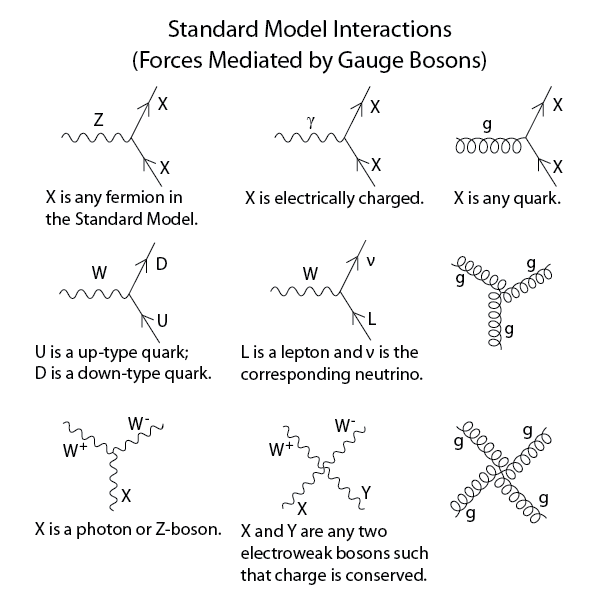
\includegraphics[width=0.75\textwidth]{Standard_Model_Feynman_Diagram_Vertices.png}
	\caption{A list of the vertices that appear in Standard Model Feynman Diagrams. Higgs Boson interactions and neutrino oscillations are omitted. Feynman rule values of the vertices are also omitted. \cite{wikipedia_SM_feynman_vertices}}
        \label{fig:SMvertices}
\end{figure}

In the SM, for processes which have longitudinally polarised W and Z bosons in the final state,
the amplitudes of the diagrams containing the Higgs Boson and of those containing TGC and QGC between electroweak bosons are separately divergent at high energies.
However, their interference between their amplitudes cancels out exactly these divergencies, maintaining the cross section finite on the whole energy spectrum.
This exact cancellation is essential to ensure the ultimate consistency of the theory, as any deviation would eventually lead to violations of the unitarity at high energies \cite{PhysRevLett.38.883}.

In the Standard Model, there are only 4 QGC allowed between electroweak bosons: $\mathrm{WWWW}$, $\mathrm{WWZZ}$, $\mathrm{WWZ\gamma}$ and $\mathrm{WW\gamma\gamma}$ (Figure \ref{fig:EWQGC}).
\begin{figure}[ht]
  \centering
  \subfigure[$\mathrm{WWWW}$]          {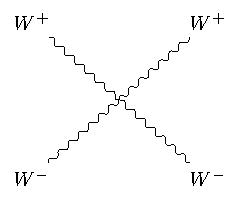
\includegraphics[width=.2\linewidth]{Figures/quartic_WWWW.pdf}}
  \subfigure[$\mathrm{WWZZ}$]          {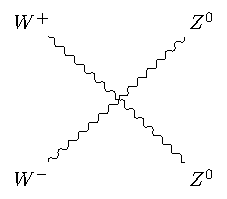
\includegraphics[width=.2\linewidth]{Figures/quartic_WWZZ.pdf}}
  \subfigure[$\mathrm{WWZ\gamma}$]     {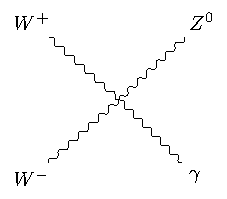
\includegraphics[width=.2\linewidth]{Figures/quartic_WWZG.pdf}}
  \subfigure[$\mathrm{WW\gamma\gamma}$]{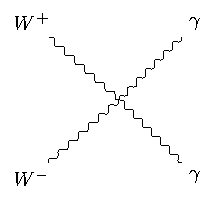
\includegraphics[width=.2\linewidth]{Figures/quartic_WWGG.pdf}}
  \caption{Electroweak Quartic Gauge Couplings allowed in the Standard Model.}
  \label{fig:EWQGC}
\end{figure}

There are several processes that are sensitive to TGCs, where their contribution is present at leading order (LO) in the perturbative calculations, but for QGC they are fewer and have very small cross sections.
One of such processes is the Vector Boson Scattering (VBS).
Another process that depends on TGC and QGC at tree level is the simultaneous production of three vector bosons.

\subsection{Triboson production at LHC}
The simultaneous production of three electroweak bosons is a class of extremely rare processes that offer an interesting insight into the mechanisms of the electroweak sector of the Standard Model.
Triboson are extremely rare events which involve the simultaneous emission of three electroweak gauge bosons -- photons, W and Z bosons -- from a single hard scattering event.
The importance of these processes is due to the fact that most of them have a significant contribution from Triple Gauge Couplings (TGC) and Quartic Gauge Couplings (QGC) at Leading Order (LO).
In particular, very few processes accessible at and hadron collider are sensitive to QGC at tree level.

A few representative Feynman diagrams for triboson production are shown in Figure \ref{fig:triboson_feynman}.
\begin{figure}[th]
  \centering
  \subfigure[]                                 {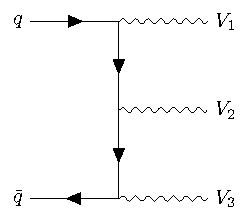
\includegraphics[width=.24\linewidth]{Figures/triboson_quarkline_VVV.pdf}}
  \subfigure[]                                 {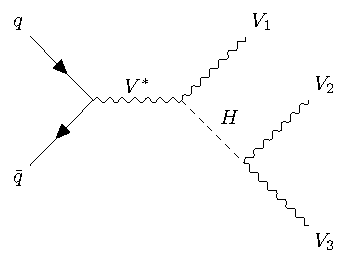
\includegraphics[width=.24\linewidth]{Figures/triboson_H_VVV.pdf}}
  \subfigure[\label{fig:triboson_feynman:TGC}] {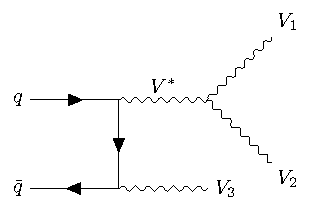
\includegraphics[width=.24\linewidth]{Figures/triboson_TGC_VVV.pdf}}
  \subfigure[\label{fig:triboson_feynman:QGC}] {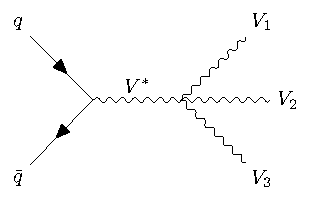
\includegraphics[width=.24\linewidth]{Figures/triboson_QGC_VVV.pdf}}
  \caption{Representative Feynman diagrams for the production of three vector bosons. Diagrams \ref{fig:triboson_feynman:TGC} and \ref{fig:triboson_feynman:QGC} are sensitive to triple and quartic gauge couplings respectively.}
  \label{fig:triboson_feynman}
\end{figure}
It must be noted that not all final states are possible through such diagrams, since charge must be conserved at each vertex, the Higgs boson does not directly couple with photons and no fully neutral vertex is allowed in the SM.
This means that no contribution from QGC (Figure \ref{fig:triboson_feynman:QGC}) is present at LO for fully neutral final states such as \PZ\PZ\PZ, \PZ\PZ\PGg, \PZ\PGg\PGg.

It offers the opportunity to test the predictions of the Standard Model with unparalleled precision in a complementary way with respect to the study of the Higgs Boson.

Due to the strikingly low cross section the study of these processes is extremely challenging,
although some have final states with a very low background.

\begin{table}[ht]
  \centering
  \caption{Summary of ATLAS and CMS results on triboson production.}
  \label{tab:summary_triboson_papers}
  \renewcommand{\arraystretch}{1.5} % more space between rows in the main table
  \begin{tabular}{l l r l}
    % the nested tables use the normal spacing
    \toprule
    Experiment & Channel(s) & Energy & Significance \\
    \midrule
    ATLAS \cite{STDM-2013-05} & $W\gamma\gamma$                &  8 TeV & $> 3 \sigma$                              \\ \hline
    ATLAS \cite{STDM-2014-01} & $Z\gamma, ZZ\gamma$            &  8 TeV & $ZZ\gamma$: 6.3 $\sigma$                  \\ \hline
    ATLAS \cite{STDM-2015-07} & $WWW$                          &  8 TeV & 0.96 $\sigma$                             \\ \hline
    ATLAS \cite{STDM-2016-05} & $WW\gamma, WZ\gamma$           &  8 TeV & $WW\gamma$ \small{(lept.)}: 1.4 $\sigma$  \\ \hline
    ATLAS \cite{STDM-2016-06} & $\gamma\gamma\gamma$           &  8 TeV & MC overestimate                           \\ \hline
    CMS   \cite{SMP-15-008}   & $W\gamma\gamma, Z\gamma\gamma$ &  8 TeV & \renewcommand{\arraystretch}{1.}\begin{tabular}{@{}l@{}}
      $W\gamma\gamma$: 2.6 $\sigma$\\ $Z\gamma\gamma$: 5.9 $\sigma$
    \end{tabular} \\ \hline
    ATLAS \cite{STDM-2017-22} & $WWW, WWZ, WZZ$                & 13 TeV & \renewcommand{\arraystretch}{1.}\begin{tabular}{@{}l@{}}
      \textbf{combined}: 4.1 $\sigma$\\ WWW \small{(lept.+semilept.)}: 3.2 $\sigma$\\ WVZ \small{(lept.+semilept.)}: 3.2 $\sigma$
    \end{tabular} \\ \hline
    ATLAS \cite{HDBS-2019-16} & $WWW$                          & 13 TeV & 8 $\sigma$, excess over SM at 2.6 $\sigma$\\ \hline
    ATLAS \cite{STDM-2021-09} & $Z\gamma\gamma$                & 13 TeV &                                           \\ \hline
    CMS   \cite{SMP-17-013}   & $WWW$                          & 13 TeV & 0.6 $\sigma$                              \\ \hline
    CMS   \cite{SMP-19-014}   & $WWW, WWZ, WZZ, ZZZ$           & 13 TeV & \renewcommand{\arraystretch}{1.}\begin{tabular}{@{}l@{}}
      \textbf{combined}: 5.0 $\sigma$\\ WWW: 2.5 $\sigma$\\ WWZ: 3.5 $\sigma$\\ WZZ: 1.6 $\sigma$\\ ZZZ: 0 $\sigma$
    \end{tabular} \\ \hline
    CMS   \cite{SMP-19-013}   & $W\gamma\gamma, Z\gamma\gamma$ & 13 TeV & \renewcommand{\arraystretch}{1.}\begin{tabular}{@{}l@{}}
      $W\gamma\gamma$: 3.1 $\sigma$\\ $Z\gamma\gamma$: 4.8 $\sigma$
    \end{tabular} \\
    \bottomrule
  \end{tabular}
\end{table}
% CMS
% SMP-15-008 & WGG, ZGG           &  8 TeV & WWG: 2.6, ZGG: 5.9                                  & http://dx.doi.org/10.1007/JHEP10(2017)072
%
% SMP-17-013 & WWW                & 13 TeV & 0.6 sigma                                           & http://dx.doi.org/10.1103/PhysRevD.100.012004
% SMP-19-014 & WWW, WWZ, WZZ, ZZZ & 13 TeV & combined: 5.0, WWW: 2.5, WWZ: 3.5, WZZ: 1.6, ZZZ: 0 & http://dx.doi.org/10.1103/PhysRevLett.125.151802
% SMP-19-013 & WGG, ZGG           & 13 TeV & WGG: 3.1, ZGG: 4.8                                  & http://dx.doi.org/10.1007/JHEP10(2021)174
%
% SMP-22-006 & WWG, HG            & 13 TeV & 5.6 sigma                                           & submitted https://cds.cern.ch/record/2875047
%
%
% ATLAS
% STDM-2013-05 & WGG           &  8 TeV & evidence, cross section & https://journals.aps.org/prl/abstract/10.1103/PhysRevLett.115.031802
% STDM-2014-01 & ZG, ZZG       &  8 TeV & 6.3 sigma               & https://journals.aps.org/prd/abstract/10.1103/PhysRevD.93.112002
% STDM-2015-07 & WWW           &  8 TeV & 0.96 sigma              & https://link.springer.com/article/10.1140/epjc/s10052-017-4692-1
% STDM-2016-05 & WWG, WZG      &  8 TeV & WWG(lept): 1.4 sigma    & https://link.springer.com/article/10.1140/epjc/s10052-017-5180-3
% STDM-2016-06 & GGG           &  8 TeV & MC overestimate         & https://www.sciencedirect.com/science/article/pii/S0370269318302533
%
% STDM-2017-22 & WWW, WWZ, WZZ & 13 TeV & & https://www.sciencedirect.com/science/article/pii/S0370269319306355
% HDBS-2019-16 & WWW           & 13 TeV & 8 sigma, excess at 2.6 sigma & https://journals.aps.org/prl/abstract/10.1103/PhysRevLett.129.061803
% STDM-2021-09 & ZGG           & 13 TeV & & https://link.springer.com/article/10.1140/epjc/s10052-023-11579-8
%
% STDM-2018-33 & WGG           & 13 TeV & & submitted https://atlas.web.cern.ch/Atlas/GROUPS/PHYSICS/PAPERS/STDM-2018-33
% STDM-2019-17 & WZG           & 13 TeV & & submitted https://atlas.web.cern.ch/Atlas/GROUPS/PHYSICS/PAPERS/STDM-2019-17

Triboson production in proton-proton collisions has been observed by both the ATLAS and CMS collaborations at LHC in several channels.
The first results were obtained during Run1 at a centre-of-mass energy of 8 TeV.

% Many articles only report a fiducial cross section, so it is more difficult to compare between experiments
% GGG
The production of three photons, $\gamma\gamma\gamma$, was observed by ATLAS \cite{STDM-2016-06}, with a measured cross section of $72.6 \pm 6.5 \text{(stat)} \pm 9.2 \text{(syst)}~\text{fb}$.
% WGG
Evidence for the production of $W\gamma\gamma$ was found by ATLAS \cite{STDM-2013-05} measuring a cross-section of $6.1^{+1.1}_{-1.0} \text{(stat)} \pm 1.2 \text{(syst)} \pm 0.2 \text{(lumi)}~\text{fb}$ for the leptonic channel,
while CMS \cite{SMP-15-008} measured $4.9 \pm 1.4 \text{(stat)} \pm 1.6 \text{(syst)} \pm 0.1 \text{(lumi)}~\text{fb}$.
% ZGG
Both ATLAS \cite{STDM-2014-01} and CMS \cite{SMP-15-008} observed $ZZ\gamma$, measuring fiducial cross sections of
$6.2^{+1.2}_{-1.1} \text{(stat)} \pm 0.4 \text{(syst)} \pm 0.1 \text{(lumi)}~\text{fb}$ for the former,
and $12.4 \pm 1.4 \text{(stat)} \pm 1.8 \text{(syst)} \pm 0.3 \text{(lumi)}~\text{fb}$ for the latter for the leptonic decay of the Z boson.
% WWG
ATLAS failed to found evidence for $WW\gamma$ \cite{STDM-2016-05}, but measured $\sigma(pp \rightarrow e\nu \mu\nu \gamma) = 1.5 \pm 0.9 \text{(stat)} \pm 0.5 \text{(syst)}~\text{fb}$.
% WWW
Similarly, ATLAS set an upper limit of 730 fb \cite{STDM-2015-07} on the cross section of $W^{\pm}W^{\pm}W^{\mp}$ at 95 \% confidence level.
% by considering two decay channels, the fully leptonic $W^{\pm}W^{\pm}W^{\mp} \rightarrow \ell^{\pm} \nu \ell^{\pm} \nu \ell^{\mp} \nu$
% and the the semileptonic $W^{\pm}W^{\pm}W^{\mp} \rightarrow \ell^{\pm} \nu \ell^{\pm} \nu j j$.

In Run2, with more statistics and also the higher centre-of-mass energy of 13 TeV, more channels became accessible.
% WGG
CMS found evidence for $W^\pm\gamma\gamma$ \cite{SMP-19-013} and measured a fiducial cross section of
$13.6^{+1.9}_{-1.9} \text{(stat)} {}^{+4.0}_{-4.0} \text{(syst)} \pm 0.08 \text{(PDF + scale)}~\text{fb}$.
% ZGG
ATLAS observed $Z\gamma\gamma$ \cite{STDM-2021-09} and measured the fiducial cross section $\sigma_{Z(\rightarrow \ell\ell)\gamma\gamma} = 2.45 \pm 0.20 \text{(stat)} \pm 0.22 \text{(syst)} \pm 0.04 \text{(lumi)}~\text{fb}$,
while CMS found evidence for the process \cite{SMP-19-013} and measured $5.41^{+0.58}_{-0.55} \text{(stat)} {}^{+0.64}_{-0.70} \text{(syst)} \pm 0.06 \text{(PDF + scale)}~\text{fb}$.
% VVV
ATLAS found evidence \cite{STDM-2017-22} and CMS observed \cite{SMP-19-014} the production of three massive vector bosons by combining multiple channels.
The former analysis considered $WWW$ and $WWZ$, finding evidence also for the two process separately and measuring inclusive cross sections
$\sigma_{WWW} = 0.65^{+0.16}_{-0.15} \text{(stat)} {}^{+0.16}_{-0.14} \text{(syst)}~\text{fb}$ and
$\sigma_{WWZ} = 0.55 \pm 0.14 \text{(stat)} {}^{+0.15}_{-0.13} \text{(syst)}~\text{fb}$ respectively.
The latter combined $WWW$, $WWZ$, $WZZ$ and $ZZZ$, measuring and inclusive cross section of $1010^{+210}_{-200}\text{(stat)}{}^{+150}_{-120}\text{(syst)}~\text{fb}$.
The individual $WWW$ and $WWZ$ channels also passed the threshold for evidence, and their cross section were measured as
$\sigma_{WWW} = 590 ^{+160}_{-150} \text{(stat)} {}^{+16}_{-130} \text{(syst)}~\text{fb}$ and
$\sigma_{WWZ} = 300 ^{+120}_{-100} \text{(stat)} {}^{+50}_{-40 } \text{(syst)}~\text{fb}$ respectively,
while for $WZZ$ the significance was lower than 3 standard deviations with a measured
$\sigma_{WZZ} = 200 ^{+160}_{-110} \text{(stat)} {}^{+70}_{-20 } \text{(syst)}~\text{fb}$,
and for $ZZZ$ only an upper limit of $\sigma_{ZZZ} < 200~\text{fb}$ at 95 \% CL could be placed.
% WWW
In another paper, ATLAS observed $WWW$ production \cite{HDBS-2019-16}, with a small excess, measuring an inclusive cross-section of $820 \pm 100 \text{(stat)} \pm 80 \text{(syst)}~\text{fb}$.
